% Patch Lifecycle Manual
\documentclass [twoside,12pt] {report}
\usepackage {showlabels}
\usepackage {xspace}
\usepackage {url}
\usepackage {fancyvrb}
\usepackage {indentfirst}
\usepackage {makeidx}
\usepackage [dvips] {graphicx}
\usepackage [left=1.25in, right=1.25in, top=1.0in, bottom=1.0in]{geometry}
\usepackage {hyperref}

% To include EPS graphics
%\begin{figure}
%\begin{center}
%\includegraphics[key=value,...]{filename}

\makeindex
\pagestyle{headings}

\begin {document}

\title {Patch Lifecycle Manager}
\author {N. T. Dabney \and J. Lebzelter}

\maketitle 
\tableofcontents

\chapter{Introduction}
\section{Patch Lifecycle Manager}
This manual covers the Patch Lifecycle Manager (\emph{PLM}).  The PLM is a system
for managing not only patches against a source tree but meta-data concerning
those patches as well.

The PLM can also run some limited tests against code submitted to the system to 
look for errors in code submissions.

\subsection{Patch Formats}
The format for patches is the accepted standard \emph{diff(1)} format.  The PLM
is not affected by the tools used to control the management of the source code
as long as patches in \emph{diff(1)} format can be generated.

Example:
\begin{verbatim}
diff -urN file.orig file.changed > file_version.patch
\end{verbatim}

\subsection{Scope}
\index{SCCS}
Most current SCCS systems allow the import and export of patches in diff format.
This common functionality allows the PLM to act as a sort of glue, enabling a
command presentation format separate from the software and formats used to manage 
the source code during development.

The PLM does not attempt to take on the role of a traditional SCCS system and 
considers managing the actual changes to individual source code files to be outside
it's area of interest.  The PLM is not well suited for SCCS work but is very well
suited as a value add to an environment where traditional SCCS tools are in place.

\subsection{Filters}
\index{Filters}
Filters are one of the powerful portions of the PLM.  A filter is essentially a 
scripted test that is run against a patch.  A filter could do anything from 
test the correct application of a patch to compile the resulting source.  A filter
could even be written to run a static profiler, lint analysis or other static analysis.
The one restriction that the filter environment has is the system cannot 
be rebooted as part of the filter test sequence.

\section{License}
\subsection{The Patch Lifecycle Manager software}
Copyright \copyright 2002-2003 Open Source Development Lab

This program is free software; you can redistribute it and/or modify
it under the terms of the GNU General Public License as published by
the Free Software Foundation; either version 2 of the License.

This program is distributed in the hope that it will be useful,
but WITHOUT ANY WARRANTY; without even the implied warranty of
MERCHANTABILITY or FITNESS FOR A PARTICULAR PURPOSE.  See the
GNU General Public License for more details.

You should have received a copy of the GNU General Public License
along with this program; if not, write to the Free Software
Foundation, Inc., 675 Mass Ave, Cambridge, MA 02139, USA.

\subsection{Changes}
Please send suggested changes to the maintainer at testdev@osdl.org.


\chapter{Using the PLM}
\section{Process}
\subsection{Lifecycle of a Patch}
The lifecycle of a patch involves numerous stages:

\begin{itemize}
\item Creation of the patch (in diff format)
\item Submission to the PLM 
\item Filter application \& reporting
\item Testing (http://www.osdl.org/stp/)
\end{itemize}

\subsection{Base Version}
\index{Base Version}
A base version is special in that it does not have any content stored in 
PLM and does not apply to any parent version.  Instead the PLM holds an 
internal pointer to where the tarball can be retrieved by utilities to be
used as the base to apply other patches onto.

The PLM has a utility that will auto-submit software versions from a web 
accessible directory structure.  These patches are added with enough 
meta-data that other utilities will be able to find the correct .tar.gz 
or .tar.bz2 file when attempting to build the source tree.

Users cannot add base versions through any of the standard interfaces.  
Currently, they may be pulled from a web-based source repository.  The 
head of this
repository is configured in the plm\_source table.  Specific directions
are then set up in the 'plm\_source\_sync' table.  This is a bit 
complicated and 
needs to be done by an admin.  The same system can be used to pull 
patches posted at the repository.

Formerly, a base version had to be created by packaging up a full source 
tree and placing it in the local directory structure that was also 
available via web.  Now, you can point at a remote URL, but keep in mind 
that this system will have the frailties of using a remote sight and 
of not controlling when files may be rearranged.  The tar archive will be 
pulled from this location every time it is accessed.  This may be best for 
testing or for systems that are not heavily used.

At the OSDL we choose to have a local mirror of the Linux Kernel ftp archive.  
When a new kernel is released, the mirror places it in the local repository.  
Then the utility notices the new version and adds the new base version to 
the PLM repository.  This is a completely automatic procedure for us.

\subsection{Apply Trees}
\index{Apply Tree}
A patch tree can be created by applying patches to base versions or previously
submitted patches.  Note that a patch can only apply to a single lower version.  
The tree can be walked to find the base version.  Using this tree structure the
back-end can build a full source tree with applied patches to use for testing.

After the initial submission to the PLM, the patch can be used as a parent
in the applies tree of another patch.  When this happens, a patch may no 
longer be deleted from the system without first deleting all of the patches 
that depend on it.

\subsection{Submission}
\index{Patch Submission}
Submission to the PLM can happen through a number of interfaces.  The basic
information that must be provided about the patch at submission time is:

\begin{itemize}
\item Name of patch
\item Name or ID of version that patch applies to
\item Actual patch content
\end{itemize}

As you can see the initial submission does not contain a large amount of 
information regarding the patch.  Most of the information the PLM keeps 
regarding patches is gathered by the system through filter runs and various
tracking information such as submission date and a md5sum of the patch.

After patch submission, a series of filters (if available) are automatically 
queued to run against the patch.  The most basic filter we run is to test
that the patch actually applies to the version specified for it.  This 
is the minimal check that should be run on all patches submitted.

\subsection{Filters}
\index{Filters}
A filter is a script that does 'something' with a patch or against the 
full source tree created from a patch applies tree.  

Filters can be created to handle any task that does not require rebooting the 
machine the filter is running on.  Some of the filters we use at the OSDL to
check Linux Kernel patches include patch application checks as well as 
multiple compilation checks for multiple architectures.  The filters have the
ability to configure a kernel for compilation, execute the compilation and
verify a correct completion.  Another compilation test counts the build warnings 
and errors and reports on those instead of the basic pass/fail.

The output of filter runs is available through the web interface on the Patch
Info page.

Filters are run automatically by the back-end and users will receive an email 
notifying them when all of the filters against the patch are complete.

\subsection{Testing}
\index{Testing}
The PLM was created to service the need of the Scalable Test Platform.  The STP
had used CVS for it's patch submissions and required users to import entire CVS
versions of the source tree in a long and painful process.

After a patch is in the PLM, if there is an associated STP setup like there is
at the OSDL, additional testing can happen there.  The STP has the ability to 
run stress tests, workloads, regression tests in a much more flexible environment 
than the PLM filters.  STP tests start out with a complete OS install and are able
to deal with system crashes and reboots during testing.

Some software (such as kernels) cannot be installed without a reboot.  These 
software items cannot be fully tested within the PLM filter framework because 
filters cannot reboot the machine to install the software.  These types of software
packages can instead be tested by the Scalable Test Platform which integrates with
the PLM to provide additional testing flexibility.

\subsection{Patch Archive}
\index{Patch Archive}
The PLM will store patches until they are deleted.  There is no automatic purge operation.

In the future, we may look at ways of decreasing the amount of storage required 
by the back-end. The current .bz2 format does keep the individual patches small but the 
uncompress time slows things down.

Patches can be deleted by the user who submitted them.  When a user is logged in and a
patch can be deleted, a link to do so will be on the Patch Info page.  Patch deletion 
can only happen through the web interface.  If there are any other patches in the system 
that apply to the patch a user wishes to delete, those dependent patches must first be 
deleted.  If they are owned by other users, the user will not be able to resolve the
dependencies and will be unable to delete the patch from the system.

There is no automatic method for deleting STP test requests that refer to a patch ID 
that has been deleted.  It is for this reason we suggest not deleting patches if you have 
requested testing through the STP system.

\section{Interfaces}
\subsection{Web Interface}
\index{Web Interface}
The main interface for the PLM is provided by a web application.  The web 
application allows users to add/delete their own patches as well as view 
information on patches already in the database.  A search interface is also 
available.

\subsubsection{Home Page}
\index{Web Interface!Home Page}
The home page provides some basic information about the PLM and provides links to
HOWTO information.  The user navigates to the rest of the main pages through the 
buttons on the top navigation bar.

\begin{center}
\scalebox{0.75}{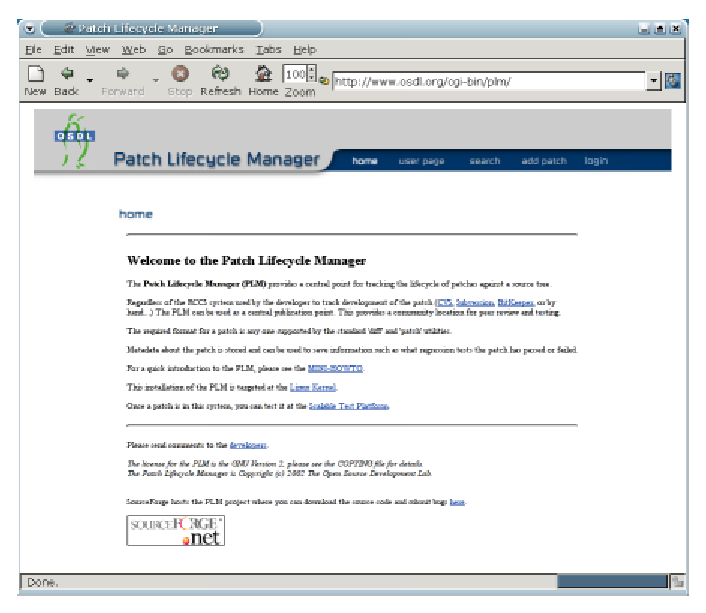
\includegraphics{images/home_page.ps}}
\end{center}

\subsubsection{User Page}
\index{Web Interface!User Page}
The user page provides a quick activity summary for an authenticated user.
Information provided includes the users login name, email address and a search 
report on the most recent patches submitted by the user.

\begin{center}
\scalebox{0.75}{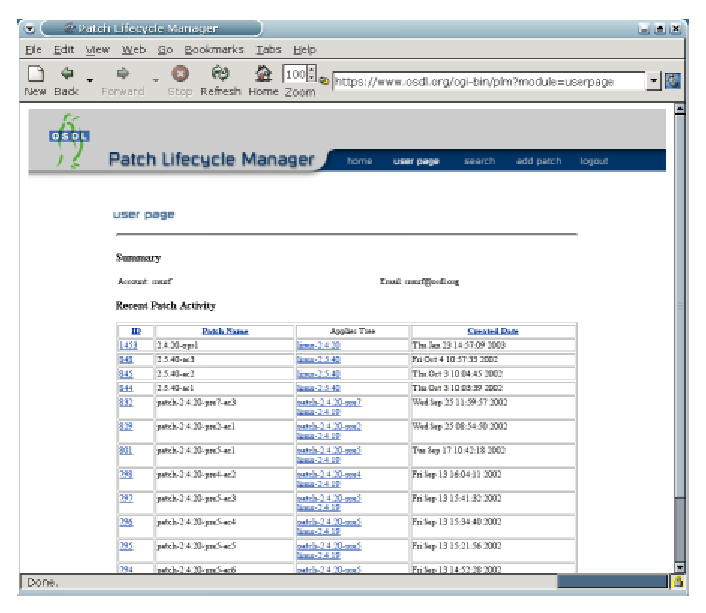
\includegraphics{images/user_page.ps}}
\end{center}

\subsubsection{Search Page}
\index{Web Interface!Search Page}
The search page provides an easy interface for finding both base software 
versions and patches.  The potential search parameters are:

\begin{itemize}
\item Patch \emph{name} or \emph{ID}
\item Name of the submitter
\item Creation date (selection from a drop-down box of possible values)
\end{itemize}

\begin{center}
\scalebox{0.75}{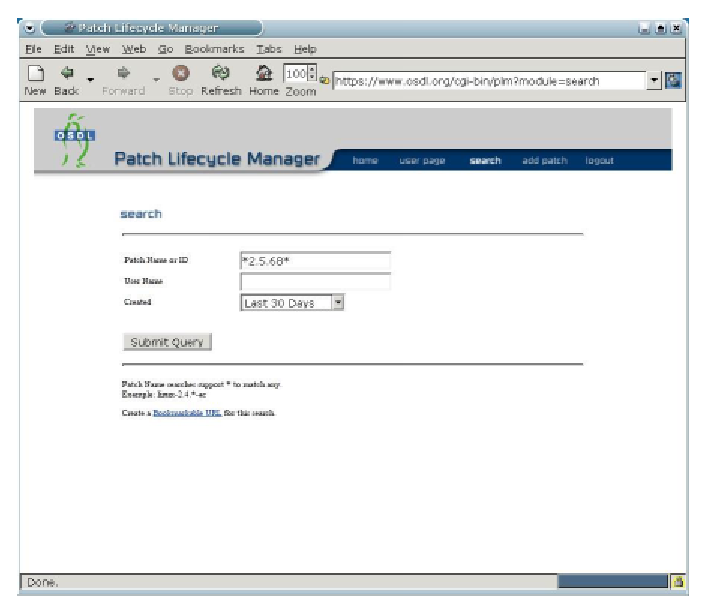
\includegraphics{images/search_page.ps}}
\end{center}

The results of the search will have hyperlinks to the \emph{Patch Information
Page} of each patch listed as well as the patches in their respective applies 
tree.

\begin{center}
\scalebox{0.75}{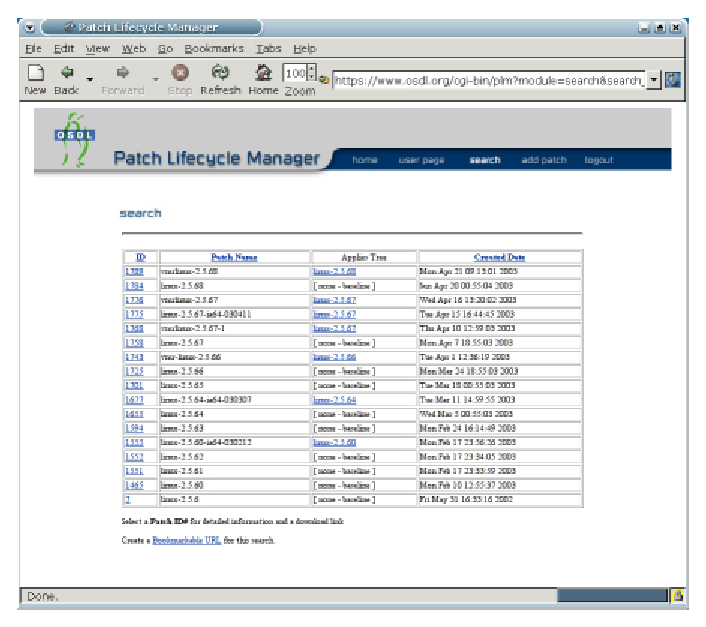
\includegraphics{images/search_results_page.ps}}
\end{center}

\subsubsection{Login Page}
\index{Web Interface!Login}
Anytime you either select the login button on the top menu, or select a page that 
requires a login, you will be prompted for your username and password.

\begin{center}
\scalebox{0.75}{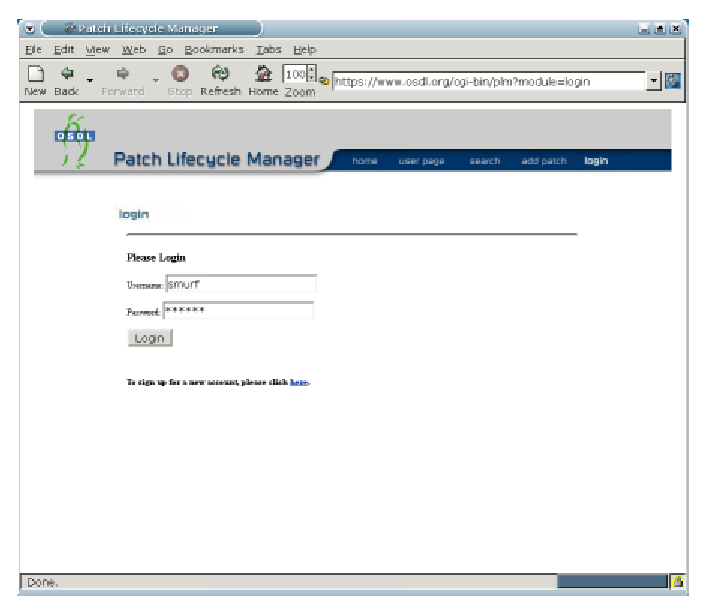
\includegraphics{images/login_page.ps}}
\end{center}

\subsubsection{Add Patch Page}
\index{Web Interface!Add Patch}
The add patch page provides a quick interface for adding new patches into the
system.  The user is required to provide the following information:

\begin{itemize}
\item Name of patch
\item Name or ID of patch to apply to
\item Content (provided by file-upload)
\end{itemize}

\begin{center}
\scalebox{0.75}{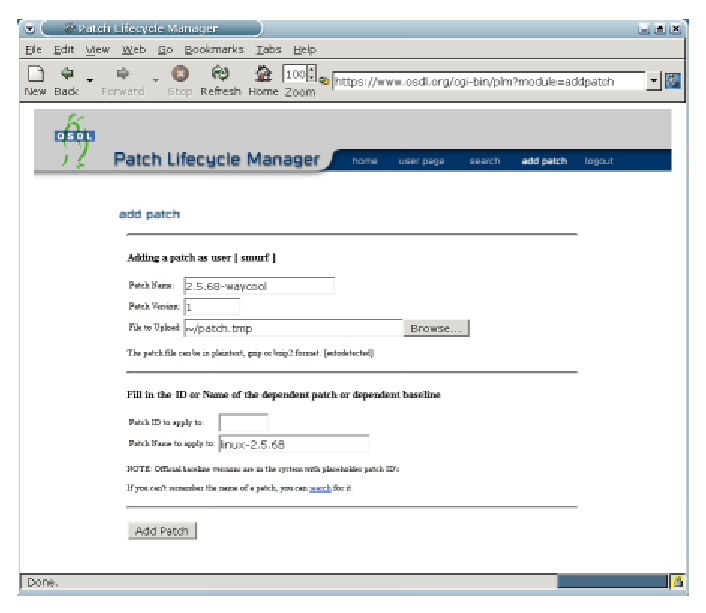
\includegraphics{images/add_patch_page.ps}}
\end{center}

The PLM system has a single namespace.  That namespace may have regions 
protected for submission by specified users.  If your patch name steps on one
of these protected regions, you will be notified.  These regions are usually
used to protect official version names.

\subsubsection{Patch Information Page}
\index{Web Interface!Patch Information Page}
The patch information page provides a detailed listing of information regarding
a patch in the PLM system.  

If the version is a base version, a pointer to an external location where the 
user can find the patch is provided.  If the version is a regular patch then 
the user can download the patch from the PLM system.  The user also has the 
options to view the patch in plain text or in code2html output with color 
highlighting.

Information available in the patch information page includes:

\begin{itemize}
\item Original submitter of the patch
\item Submission date \& time
\item The name of the patch
\item md5sum \index{md5sum} of the patch
\item Patch Applies tree with links to relative patch information pages
\item Report on filter results (if available)
\end{itemize}

\begin{center}
\scalebox{0.75}{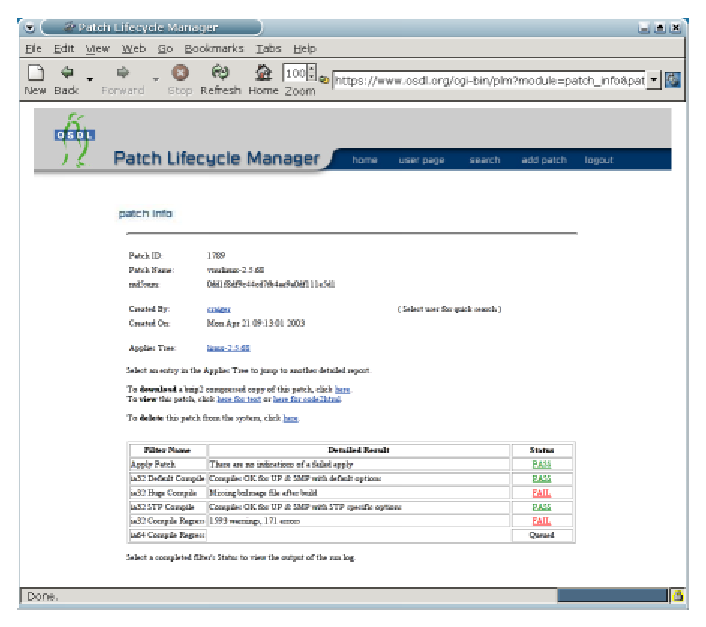
\includegraphics{images/patch_info_page.ps}}
\end{center}

\subsection{Email Interface}
\index{Email Interface}
An email gateway is available with a subset of the web interface's 
functionality. The email gateway can be used by command line scripts for easy 
SCCS=$>$PLM \footnote{The SCCS=$>$PLM gateways will be SCCS specific and have 
not been written yet.} gateway functionality.

The functionality of the email gateway is currently limited to the submission of
new patches.  Patches submitted through the email gateway need to have a limited
amount of meta-data in a special \emph{plm header} to designate parameters such
as the name of the patch and the PLM ID of the baseline or patch that the 
submitted patch applies to.

\subsubsection{Email Gateway Metadata}
\index{Email Interface!Metadata}

If you use the plmsend script, you do NOT NEED to understand this section.

Actions on patches sent in to the PLM are determined by metadata tags included at
the top of the patch in comments. To use a metadata tag, put it at the start of
the patch in the following form: 
	
	\#plm $[$metadata-tag$]$ $[$options...$]$

Each patch has metadata parameters, some are required and some are optional.  
Metadata is included as comments to the patch, for example:

contents of kernel.patch:
\begin{verbatim}
#plm login example-username example-password 
#plm name 2.4.18-rc2 
#plm applies linux-2.4.17
diff -Naur -X /home/marcelo/lib/dontdiff linux.orig/CREDITS linux/CREDITS
\end{verbatim}

The diff line is the start of the actual patch and the \#plm lines will be 
stripped before the patch is saved.

The required lines are:
\begin{itemize}
\item login $[$username$]$ $[$password$]$
\item name "string name for patch"
\item applies "name of the patch or regular version this applies to"
\end{itemize}

Email your patch file (with the metadata included) to the submission address for
the repository you are working with.

You will get an email in response telling you the PLM ID of the accepted patch 
or telling you what went wrong with your submission.  If you don't get any 
email back at all, that means you don't have an account.  We don't respond to 
invalid account emails to avoid being triggered by SPAM.  \footnote{In the future if you 
attempt to login with a '\#plm login' command and your login fails, we will 
email you to let you know.}

Security is obviously an issue when you are sending usernames and passwords
over the Internet.  To keep your information secure, the email interface supports
encryption using the gnupg program available at: http://www.gnu.org/directory/gnuPG.html

\subsection{plmsend script}
\index{Email Interface!plmsend}
'plmsend' is a script for auto-submission of patches.  It will handle the 
encryption and patch metadata information for you.

After downloading the plmsend script, you will want to create a ~/.plmrc file.
The format of this file is as follows:

VARIABLE=VALUE where VARIABLE can be any of:
\begin{itemize}
\item USER - For your username on the PLM system
\item PASS - For your account (make sure the file is readable only by you if
         you include this)
\item PLM\_TO\_ADDR - The email address to submit patches to.  Set this to
PLM\_TO\_ADDR=plm@osdl.org
\end{itemize}
(the following options are optional)

\begin{itemize}
\item ENCRYPT - Encryption is on by default, to disable it, set this to 'off'
\item MAILER - Tell the script to use either 'mail' or 'mutt' to compose the email
\item SANITY - If you don't want to hit enter to confirm a submission, set:
           'SANITY=gone'
\end{itemize}

After you have a valid ~/.plmrc file and have a patch ready, remember you need
to have the following information:

\begin{itemize}
\item Applies - You need to know the patch name that your patch applies to (as
registered in the PLM database).  For regular mainline Linux Kernel
patches, the naming looks /exactly/ like the file on kernel.org
example:  linux-2.4.18  or  patch-2.4.19-pre2
\item Name - Your patch needs a name - include the version in the string.
\item Filename - The name of your file on disk.  If you can't find this, I can't
             help you.
\end{itemize}

Syntax for the plmsend command is:

\begin{verbatim}
plmsend <applies> <name> <filename>
\end{verbatim}

Example plmsend submission command:

\begin{verbatim}
$ plmsend linux-2.4.18 2.4.18-rawio-2 2.4.18-rawio-2.patch
\end{verbatim}
  
\subsection{RPC Interface}
\index{RPC Interface}
There is a limited XML/RPC interface for remote applications.  This interface 
is the one that future command line client scripts will use to interact with 
the main system.

The email gateway is one such remote interface.  It uses the RPC interface as a 
remote back-end for it's library functions.

Authentication is built into the RPC schema to allow the email gateway to run 
in untrusted environments.  There is also a trusted version of the RPC 
interface for environments where security is not an issue.



\chapter{Installation}
The installation of the Patch Lifecycle Manager is involves a lot of details.  The system runs fairly well on it's own once everything is setup and configured correctly.
\section {Downloading the PLM}
\index{Downloading the PLM}
We currently make the tarball sources available.  This includes a script called lsb\_package.sh which when run will generate a RedHat rpm, tested on 8.  The spec file, 'lsb-rpm.spec', is in the top directory.  Or you can download the rpm we generate at the URL listed below, but it places the items in set locations. 

If you would like to assist us with providing build patches for other targets, please feel free to contribute.

The source for the Patch Lifecycle Manager is located at:
\url{http://www.osdl.org/archive/plm/Source/}

The RedHat 8.0 RPM packages for the Patch Lifecycle Manager are located at:
\url{http://www.osdl.org/archive/plm/RPM}

\section {Installing the RPM}
\index{Install}

\subsection{RPM Dependencies}
\index{Install!RPM Dependencies}
The dependencies for the PLM depend on what type of host you are installing the RPM on (aka, what it's going to be used for)
In the future we plan to split out the RPM into the various uses and have rpm handle the dependency issues for us.

For CVS access, the following perl modules are required:  IO-Tty-1.02 (for Pty), Class-Accessor-0.19, IPC-Run-0.78, Cvs-0.06.  (The version numbers are just what I used, maybe older ones will work, except for Cvs where only 0.06 or better will work).


\subsection{Perl Dependencies}
\index{Install!Perl Dependencies}
For a PLM Supervisor client host, you only need the Mail::Internet perl module.

\subsection{Configuration}
The configuration file for the PLM is /etc/plm.cfg.  Each type of server/client will have different portions of that file that are important to it.  Those will be listed under their own configuration sections.

\subsection{Bug Workarounds}
\index{Install!Bug Workarounds}
The following bug workarounds are suggested:

\begin{itemize}
\item The file /var/log/plm.log must be created and writable by whatever user your PLM scripts will be run as.  In the future we plan to move all the logging to a syslog USER* facility.
\item You may need to force-nodeps to get the RPM to install
\end{itemize}

\section {PLM Host Types}

\index{Admin!HostType}
PLM will usually be installed on several machines which can generally be classified by functionality.

\begin{itemize}
\item Web Server:  Provide access to the patches, and database through ASP functions.
\item Simple Client: Provide access to patches
\item Supervisor Client: Processes filters for the patches
\item Administrative Client: Run various administrative scripts
\end{itemize}

Some of the hosts may serve more than one purpose.  They should be configured according only to their purpose, or the configuration file will get confusing, as well as contain more sensitive information than necessary.

\section {General Configuration of PLM Host}

\subsection{General Configuration}
\index{Configure!General!Configuration}
The entries in the /etc/plm.cfg file for any PLM Host are:

\begin{itemize}
\item log\_file: 
\item log\_target: 
\item log\_level:
\end{itemize}

\section {Configuring a Web Interface}
\index{Configure!Web Interface}
Configuring a web interface requires some additional work after the RPM is installed.

In the future, we plan to have a web interface specific RPM that does all of
the following tasks on install.

\subsection{Configuration}
\index{Configure!Web Interface!Configuration}
The important entries in the /etc/plm.cfg file for the web interface scripts are:

\begin{itemize}
\item dsn: Perl DSN (DBI:mysql:host=hostname;dbname=database)
\item dsnuser: Username to login to the database with
\item dsnpass: Password to login to the database with
\item namespace: Should be plm\_
\item plm\_http: URL for the cgi-bin space (used in links)
\item getpatch\_url: Full URL to the getpatch script (used in links)
\item support\_email: Email address for users to send questions to
\item admin\_email: Email address to send administrator errors to
\item access\_state\_dir: On-disk location of the login cookies (pay attention to standard security precautions.  Make sure this directory is only readable by the web interface user)
\item repository\_path: Location on webserver where PLM patches are stored. Readable and writable by web owner.
\item webapp\_data\_dir: Local directory where the brand .html files are located
\item webapp\_image\_url: URL portion showing where the PLM images are kept
\item webapp\_brand: Code (used in file names) for brand identification
\item webapp\_patch\_server: Where the webapp should point people to download patches
\item webapp\_source\_\#: The webapp source link for where to get base versions for repository \# 
\item new\_account\_link: URL to send users to who need an account on the system (hey, if anybody wants to provide the PLM with it's own user management interface, that would be great.  We don't need one so we didn't write one)
\end{itemize}

\subsection{Cron Job}
\index{Configure!Web Interface!Cron Job}
The logins for the PLM do not have a default expire date.  Cookies are expired server-side by deleting their files.  Each time a user with a session access the web interface, the atime on the cookie file is updated.  A cron job should be setup to delete old cookies.  A crontab user entry could look like:

\begin{verbatim}
*/10 * * * * (cd /var/plm/access && find -amin +180 -print | xargs rm -vf)
\end{verbatim}

That would effectively purge (Every 10 minutes) the access directory of any login cookies that were older than 3 hours.  Remember, a session will last as long as a user is constantly active.  The user would have to be away from the site for 3 hours before this would take effect.

\subsection{Configuration Steps}
We suggest the following steps for setting up a supervisor system:
\begin{enumerate}
\item Perform the regular steps from 'Installing the RPM'
\item Add a 'plm' user to the system
\item Configure the /etc/plm.cfg with the proper web interface options
\item Configure the /etc/plm.cfg with the proper web user permissions
\item Configure the /var/plm/access directory
\item Configure the /var/plm/access cron job
\item Move the web interface (getpatch, plm, plm\_server.pl, asp-private) scripts to your cgi-bin directory.
\item Configure your web server to restrict access to the asp-private script (if security is a concern at this location)
\end{enumerate}

\section {Configuring a Supervisor host}
\index{Configure!Supervisor}
The supervisor script controls the execution of the filters.  

\subsection{Multiple Supervisors}
\index{Configure!Supervisor!Multiple}
If your filters are single-threaded, you can run one supervisor per CPU on the machine.
If not, then you will want to take scaling issues into account when deciding how many 
supervisors to run on each machine.  Each supervisor will require it's own scratch space.

\subsection{Scratch Space}
\index{Configure!Supervisor!Scratch Space}
The scratch space is where the supervisor downloads the software, applies patches, builds
the software and applies the filters.  Having multiple supervisors run in the save 
scratch space will cause major problems.  To avoid this, the supervisor script takes a
'lockfile' command line option.  Pick a filename (such as PID) and use it for every
supervisor on the machine to avoid accidental issues.

\subsection{Supervisor Configuration}
\index{Configure!Supervisor!Configuration}
The supervisor hosts will also act as clients, so in addition to the following configuration parameters for a client should be set up. The important entries in the /etc/plm.cfg file for the asp\_supervisor.pl script are:

\begin{itemize}
\item ccache\_dir: Specifies where to store the ccache work files
\item supervisor\_sleep: Number of seconds to sleep between polling for new filters
\item filter\_type: Types of filters this supervisor can run (: delimited)
\end{itemize}

\subsection{Cron Job}
\index{Configure!Supervisor!Cron Job}
The cronjob for each supervisor you wish to run on the machine should do the following two things:

\begin{enumerate}
\item Change into the scratch
\item Launch the asp\_supervisor.pl script
\item Provide the asp\_supervisor.pl script with the lock filename
\item Redirect the output from asp\_supervisor.pl script to somewhere sane
\end{enumerate}

Examples:
\begin{verbatim}
*/15 * * * * cd /home/plm/scratch/1 && asp\_supervisor.pl PID 1>> LOG 2>> LOG &
*/15 * * * * cd /home/plm/scratch/2 && asp\_supervisor.pl PID 1>> LOG 2>> LOG &
\end{verbatim}

Note: You may need the full pathname to the asp\_supervisor.pl script.  
(/usr/local/bin/asp\_supervisor.pl)

\subsection{Configuration Steps}
We suggest the following steps for setting up a supervisor system:
\begin{enumerate}
\item Perform the regular steps from 'Installing the RPM'
\item Add a 'plm' user to the system
\item Create /home/plm/scratch/[1..CPU] directories for scratch space
\item If you have multiple disks, spread the actual scratch directories around and use symlinks
\item Configure the /etc/plm with the proper supervisor-specific options
\item Configure one cron job for each scratch directory
\item Make a link called /usr/local/bin/gcc to /usr/bin/ccache
\item Install "server-dead.sh" in /home/plm.  Make sure the path is set right in the script.  Set it up as a cron job hourly.
\item (this is a bug workaround) chmod +x /usr/local/bin/asp\_supervisor.pl
\end{enumerate}

\section {Configuring a Client}

\subsection{Client Configuration}
\index{Configure!Client!Configuration}
The important entries in the /etc/plm.cfg file for the plm\_build\_tree.pl script are:

\begin{itemize}
\item PLMClient\_uri: Set to 'Base' (the name of a Perl module)
\item PLMClient\_proxy: URL or relative URL to 'plm\_private\_server.pl'
\item getpatch\_url: URL to 'getpatch' CGI script.
\end{itemize}

\subsection{Configuration Steps}
We suggest the following steps for setting up a supervisor system:
\begin{enumerate}
\item Perform the regular steps from 'Installing the RPM'
\item Add a 'plm' user to the system
\item Configure the /etc/plm with the proper client-specific options
\end{enumerate}

The system runs fairly well on it's own once everything is setup and configured correctly.  There are some routine tasks which will need to be done, and for this there are quite a few command line scripts.
\section {Adminstrative Scripts}
\index{Admin!Scripts}
These administrative scripts mostly query the database directly, by-passing the web interface and PLM methods except for the getCoonfig.  The exception to this is the plm\_source\_sync.pl which uses the ASP calls.  Most of these are little helper scripts so that an admin does not have to re-write queries or access the database.  Make sure they are not runable by all users, because they access the passwords in the plm.cfg file.  These scripts should give help if run with no options. 

\begin{itemize}
\item plm\_add\_filter.pl:  Add new filter.
\item plm\_add\_filter\_type.pl:  Add new filter type.
\item plm\_user:  Administer user accounts
\item plm\_source\_sync.pl:  Update PLM database from a source repository which is configured in tables 'plm\_source' and 'plm\_source\_sync'.  This requires its own configuration file for each source repository to be synchronised.  Can run manually, but usually will be a cron job.
\item plm\_request\_filter.pl: PLM automatically requests filters for a patch only when it is added to the system.  This script is intended to be used to request filters for a patch when the filter has been added to the system after a patch has.
\item plm\_status.pl:
\item plm\_filter\_check.pl:
\item plm\_filter\_output.pl:
\item plm\_report.pl:
\item plm\_reset\_request.pl: This is intended as a simple tool to reset a particular filter request for a patch or all filter requests for a patch to the queued state.
\item plm\_version\_sync.pl:  (replaced by plm\_source\_sync.pl)  This script updated PLM database from an archive which was on the host where was run.
\end{itemize}

\section {Configure Software}
\index{Admin!Software}
A new software type is added using the script 'plm\_add\_software.pl'.

\section {Configure Source}
\index{Admin!Source}
Once a new software is created, a 'source' for the base must be configured in table 'plm\_source'.  There is currently no script to do this, so I will mention here the important database fields.  Multiple sources and source types are possible for one software type.

\begin{itemize}
\item id: Unique integer identifier
\item plm\_software\_id: Relates back to table 'plm\_software' table
\item plm\_source\_type: Currently 'TAR', 'CVS', future 'BK' etc.
\item root\_location: Top URL for web site, for TAR
\item source\_password: Text password for access to Source Control Repository
\item sc\_module: Module name for Source control Repository
\item sc\_branch: Not implemented
\end{itemize}

\section {Configure SourceSync}
\index{Admin!SourceSync}
In order to sync using plm\_source\_sync.pl from an existing repository, at least one entry must be put into table 'plm\_source\_sync'.  The fields in this table are:

\begin{itemize}
\item id: Unique integer identifier
\item plm\_source\_id:  Relates back to table 'plm\_source'
\item search\_location:  Continuation of URL, for source type TAR
\item depth: How many directories to go down, for source type TAR values start at 0
\item wanted\_regex: A regular expression to match while searching
\item not\_wanted\_regex: A regular expression to NOT match while searching(optional)
\item baseline: 'Y' or 'N', is the file a patch or a base 
\item applies\_regex: A regular expression to match name of applies, for patches NOT bases
\item name\_substitution: a full substitution expression s/xxx/yyy/ (optional)
\item descriptor: A phrase that describes this development tree.
\item last\_timestamp: This is the timestamp for the last base item added.
\end{itemize}


For Source Type TAR, use fields id, plm\_source\_id, search\_location, depth, wanted\_regex (optional), not\_wanted\_regex (optional), baseline, applies\_regex, name\_substitution (optional), descriptor.  For Source Type CVS, use fields id, plm\_source\_id, baseline (only 'Y' supported), descriptor, last\_timestamp. 

To test your newly configured sources, you run plm\_source\_sync.pl with the --list\_only option.  It prints out what plm patches it would create.

\section {Configure plm_software_to_command_set}
\index{Admin!SourceSync}
The script plm\_source\_app.pl executes the build and installations scripts.  If none are configured, this script does not return an error.  If you want it to do something the build information must be entered into three tables:  plm\_software\_to\_command\_set, plm\_command\_set and plm\_command.  The fields in this table plm\_software\_to\_command\_set are:

\begin{itemize}
\item id: Unique integer identifier
\item plm\_software\_id:  id from table plm\_software
\item plm\_command\_set\_id:  id from table plm\_command\_set
\item min\_plm\_patch\_id:  lower bound of legitimate rage for this script
\item max\_plm\_patch\_id:  upper bound of legitimate rage for this script
\end{itemize}


Table plm\_command\_set sets up a unique id for the set in table plm\_command:
\begin{itemize}
\item id: Unique integer identifier
\item name:  Brief, user-friendly identifier
\item command\_set\_type: 'build', 'install' or 'validate'.
\end{itemize}

Table plm\_command contains the actual execution sequence and expected results:
\begin{itemize}
\item id: Unique integer identifier
\item plm\_command\_set\_id:  id from table plm\_command\_set
\item command\_order:  Order to execute in.
\item command:  Can be a executable or a script, single or multi-line.
\item command\_type:  'script' or others may be added
\item expected\_result:  For type 'script', this is the return value.

%\input{sections/database_admin.tex}
%\input{sections/email_admin.tex}
%\input{sections/web_admin.tex}
%\input{sections/rpc_admin.tex}
%\input{sections/install_checklist.tex}
%\input{sections/ts_admin.tex}

%\input{sections/database_admin.tex}
%\input{sections/email_admin.tex}
%\input{sections/web_admin.tex}
%\input{sections/rpc_admin.tex}
%\input{sections/install_checklist.tex}
%\input{sections/ts_admin.tex}

\chapter{Administration}
The system runs fairly well on it's own once everything is setup and configured correctly.  There are some routine tasks which will need to be done, and for this there are quite a few command line scripts.
\section {Adminstrative Scripts}
\index{Admin!Scripts}
These administrative scripts mostly query the database directly, by-passing the web interface and PLM methods except for the getCoonfig.  The exception to this is the plm\_source\_sync.pl which uses the ASP calls.  Most of these are little helper scripts so that an admin does not have to re-write queries or access the database.  Make sure they are not runable by all users, because they access the passwords in the plm.cfg file.  These scripts should give help if run with no options. 

\begin{itemize}
\item plm\_add\_filter.pl:  Add new filter.
\item plm\_add\_filter\_type.pl:  Add new filter type.
\item plm\_user:  Administer user accounts
\item plm\_source\_sync.pl:  Update PLM database from a source repository which is configured in tables 'plm\_source' and 'plm\_source\_sync'.  This requires its own configuration file for each source repository to be synchronised.  Can run manually, but usually will be a cron job.
\item plm\_request\_filter.pl: PLM automatically requests filters for a patch only when it is added to the system.  This script is intended to be used to request filters for a patch when the filter has been added to the system after a patch has.
\item plm\_status.pl:
\item plm\_filter\_check.pl:
\item plm\_filter\_output.pl:
\item plm\_report.pl:
\item plm\_reset\_request.pl: This is intended as a simple tool to reset a particular filter request for a patch or all filter requests for a patch to the queued state.
\item plm\_version\_sync.pl:  (replaced by plm\_source\_sync.pl)  This script updated PLM database from an archive which was on the host where was run.
\end{itemize}

\section {Configure Software}
\index{Admin!Software}
A new software type is added using the script 'plm\_add\_software.pl'.

\section {Configure Source}
\index{Admin!Source}
Once a new software is created, a 'source' for the base must be configured in table 'plm\_source'.  There is currently no script to do this, so I will mention here the important database fields.  Multiple sources and source types are possible for one software type.

\begin{itemize}
\item id: Unique integer identifier
\item plm\_software\_id: Relates back to table 'plm\_software' table
\item plm\_source\_type: Currently 'TAR', 'CVS', future 'BK' etc.
\item root\_location: Top URL for web site, for TAR
\item source\_password: Text password for access to Source Control Repository
\item sc\_module: Module name for Source control Repository
\item sc\_branch: Not implemented
\end{itemize}

\section {Configure SourceSync}
\index{Admin!SourceSync}
In order to sync using plm\_source\_sync.pl from an existing repository, at least one entry must be put into table 'plm\_source\_sync'.  The fields in this table are:

\begin{itemize}
\item id: Unique integer identifier
\item plm\_source\_id:  Relates back to table 'plm\_source'
\item search\_location:  Continuation of URL, for source type TAR
\item depth: How many directories to go down, for source type TAR values start at 0
\item wanted\_regex: A regular expression to match while searching
\item not\_wanted\_regex: A regular expression to NOT match while searching(optional)
\item baseline: 'Y' or 'N', is the file a patch or a base 
\item applies\_regex: A regular expression to match name of applies, for patches NOT bases
\item name\_substitution: a full substitution expression s/xxx/yyy/ (optional)
\item descriptor: A phrase that describes this development tree.
\item last\_timestamp: This is the timestamp for the last base item added.
\end{itemize}


For Source Type TAR, use fields id, plm\_source\_id, search\_location, depth, wanted\_regex (optional), not\_wanted\_regex (optional), baseline, applies\_regex, name\_substitution (optional), descriptor.  For Source Type CVS, use fields id, plm\_source\_id, baseline (only 'Y' supported), descriptor, last\_timestamp. 

To test your newly configured sources, you run plm\_source\_sync.pl with the --list\_only option.  It prints out what plm patches it would create.

\section {Configure plm_software_to_command_set}
\index{Admin!SourceSync}
The script plm\_source\_app.pl executes the build and installations scripts.  If none are configured, this script does not return an error.  If you want it to do something the build information must be entered into three tables:  plm\_software\_to\_command\_set, plm\_command\_set and plm\_command.  The fields in this table plm\_software\_to\_command\_set are:

\begin{itemize}
\item id: Unique integer identifier
\item plm\_software\_id:  id from table plm\_software
\item plm\_command\_set\_id:  id from table plm\_command\_set
\item min\_plm\_patch\_id:  lower bound of legitimate rage for this script
\item max\_plm\_patch\_id:  upper bound of legitimate rage for this script
\end{itemize}


Table plm\_command\_set sets up a unique id for the set in table plm\_command:
\begin{itemize}
\item id: Unique integer identifier
\item name:  Brief, user-friendly identifier
\item command\_set\_type: 'build', 'install' or 'validate'.
\end{itemize}

Table plm\_command contains the actual execution sequence and expected results:
\begin{itemize}
\item id: Unique integer identifier
\item plm\_command\_set\_id:  id from table plm\_command\_set
\item command\_order:  Order to execute in.
\item command:  Can be a executable or a script, single or multi-line.
\item command\_type:  'script' or others may be added
\item expected\_result:  For type 'script', this is the return value.

%\input{sections/database_admin.tex}
%\input{sections/email_admin.tex}
%\input{sections/web_admin.tex}
%\input{sections/rpc_admin.tex}
%\input{sections/install_checklist.tex}
%\input{sections/ts_admin.tex}

\chapter{Internals}
\section {Introduction}
    The internals of the Patch Lifecycle Manager are all written in various
shell scripts with Perl being the most common language.

The major components of the PLM are:
\begin{itemize}
\item Web Server
\item Email Gateway
\item PLM Email Client (plmsend)
\item Library
\end{itemize}

The major library layers are:
\begin{itemize}
\item Base (common)
\item PLM 
\item XML
\item DB (Abstraction)
\item ASP
\item PLMClient
\end{itemize}

\section{Web Interface}
\subsection{Web Application}
\index{Web Interface!Internals!Web Application}
The PLM web server application is served through a single cgi-bin program called \emph{plm}.

The \emph{plm} script makes use of the following standard libraries libraries:
\begin{itemize}
\item MIME::Base64
\item Fcntl
\item POSIX
\item CGI
\item CGI::Carp
\end{itemize}

The \emph{plm} script makes use of the following PLM libraries:
\begin{itemize}
\item PLM
\item PLMClient
\item PLM::Web::General
\item PLM::Web::Session
\item PLM::Web::Userpage
\item PLM::Web::Addpatch
\item PLM::Web::Patch
\end{itemize}

Web pages are organized as "modules" or "content sections".  Two of the available modules
are handled directly by the \emph{plm} script:

\begin{itemize}
\item content\_home
\item content\_filter\_output
\end{itemize}

The \emph{plm} script parses the new HTTP request from stdin and hands control
off to the correct content\_* function depending on the value of the \emph{module}
URL option.  If no module option was given, the content\_home page is served.  If
an invalid module is given a security warning is sent to syslog in the form of a 
CGI::Carp warn() message.

\subsection{ASP Server}
\index{Web Interface!Internals!ASP Server}

The regular interface for RPC calls is provided by the \emph{plm\_server.pl} script.

Authorization is handled on a as-need basis for function calls through this interface.
SSL is used as the encryption method for calls coming in through this interface.

The \emph{plm\_server.pl} script makes use of the following standard libraries:
\begin{itemize}
\item CGI::Carp
\end{itemize}

The \emph{plm\_server.pl} script makes use of the following PLM libraries:
\begin{itemize}
\item PLM::RPC::Server
\item PLM::PLM
\end{itemize}

The \emph{plm\_server.pl} script is a short one that
handles the SOAP calls.

\subsection{Private ASP Server}
\index{Web Interface!Internals!Private ASP Server}

A sub-set of RPC calls are available to trusted clients 
only through the \emph{plm\_private\_server.pl} script.  These are for use from the Supervisors.

Authorization should happen at the Web Server level because there is *zero* 
authentication built into this script.

The \emph{plm\_server.pl} script makes use of the following standard libraries:
\begin{itemize}
\item CGI::Carp
\end{itemize}

The \emph{plm\_server.pl} script makes use of the following PLM libraries:
\begin{itemize}
\item PLM::PLM
\item PLM::RPC::PrivateServer
\end{itemize}

The \emph{plm\_private\_server.pl} script is a short one that 
handles the SOAP calls.

\subsection{getpatch}
\index{Web Interface!Internals!getpatch}

The \emph{getpatch} script provides an easy URL link for downloading and 
viewing patches.  The hope is that the URL can be included in emails with
a logical formatting.

The \emph{getpatch} script makes use of the following standard CGI library 
as well as the main \emph{PLM} PLM library.

The URL parameter \emph{id} specifies the patch ID to retrieve.

The following ID extensions are supported:
\begin{itemize}
\item{.bzip2} Compressed download
\item{.html}  Pretty Printed formatting of text
\item{none}   Regular plain text download
\end{itemize}

The \emph{Content-Disposition: attachment; filename=} header is included to
tell the client that the data being downloaded should be saved to a file.

The \emph{Content-Type: application/octet-stream} header is included to tell
the client the same thing in case it didn't get it the first time.

There is no authorization on patch downloads.  If the patch exists, users 
can download it.

\subsection{PLM Report}
\index{Web Interface!Internals!plm\_report.pl}

\subsection{PLM Report Results}
\index{Web Interface!Internals!plm\_report\_results.pl}

\section{PLM Library}
\subsection{Util}
The PLM::Util:: module space has the following sub-modules:

\begin{itemize}
\item Cache.pm
\item Config.pm
\item Log.pm
\item Trace.pm
\end{itemize}

\subsubsection{Config.pm}
\index{PLM::Util::Config.pm}
Reads the configuration data from disk and provides an API for accessing it.

\begin{verbatim}
new()
\end{verbatim}
\index{PLM::Util::Config.pm!new()}
Instantiates a new object of type PLM::Util::Config.

\begin{verbatim}
file()
\end{verbatim}
\index{PLM::Util::Config.pm!file()}
Load a file, returning an associative array of values.

\begin{verbatim}
get( $key )
\end{verbatim}
\index{PLM::Util::Config.pm!get()}
Returns an option if it's defined, otherwise returns an empty string.

\begin{verbatim}
set( $key, $value )
\end{verbatim}
\index{PLM::Util::Config.pm!set()}
Sets the config option based on the key and value.

\begin{verbatim}
getKeys()
\end{verbatim}
\index{PLM::Util::Config.pm!getKeys()}
Returns a list of the keys in the config object.

\begin{verbatim}
getHash()
\end{verbatim}
\index{PLM::Util::Config.pm!getHash()}
Returns the hash reference to the internal config object keys.

\subsubsection{Log.pm}
\index{PLM::Util::Log.pm}
Provides an interface for modules \& scripts to log events.

\begin{verbatim}
new()
\end{verbatim}
\index{PLM::Util::Log.pm!new()}
Instantiates a new object of type PLM::Util::Log.

\begin{verbatim}
config( %options )
\end{verbatim}
\index{PLM::Util::Log.pm!config()}
Parses the options passes to new() or can be called after new() with additional config arguments.

\begin{verbatim}
debug( $value )
\end{verbatim}
\index{PLM::Util::Log.pm!debug()}
Sets the debug level for the object.

Debug messages are tested against this level and if they are the same level or higher, they are considered valid and set to the logging target.  Otherwise, they are ignored.

\begin{verbatim}
target( $string )
\end{verbatim}
\index{PLM::Util::Log.pm!target()}
Tells the logging subsystem where to log events.  Valid targets are:

\begin{itemize}
\item stdout
\item stderr
\item email
\item syslog
\item file
\end{itemize}

If you are setting the target to 'file' then you must first set the filename using the filename() call or an earlier config() option.

\begin{verbatim}
filename( optional: $path )
\end{verbatim}
\index{PLM::Util::Log.pm!filename()}
Gets or sets the filename to be used as the log target.  If the filename is not passed to the function, the function only returns the current setting.

\begin{verbatim}
mylog( $level, $text )
\end{verbatim}
\index{PLM::Util::Log.pm!mylog()}
Checks to see if the log message is of a high enough priority and if so, logs it to the log target.

\begin{verbatim}
msg()
\end{verbatim}
\index{PLM::Util::Log.pm!msg()}
Wrapper call for mylog() - no, I don't know why we have two either.

\subsubsection{Trace.pm}
\index{PLM::Util::Trace.pm}
Provides a generic panic and error handling routines to the PLM modules.

\begin{verbatim}
trace_configure( $log_ref, $config_ref )
\end{verbatim}
\index{PLM::Util::Trace.pm!trace\_configure()}
Takes a reference to a PLM::Util::Log object and a reference to a PLM::Util::Config 
object for later use.

\begin{verbatim}
panic( $reason_txt )
\end{verbatim}
\index{PLM::Util::Trace.pm!panic()}
Calls the call\_trace routine with the proper options to do a call trace and 
to follow with a panic.

\begin{verbatim}
call_trace( $reason_txt, $panic_trigger )
\end{verbatim}
\index{PLM::Util::Trace.pm!call\_trace()}
Generates a call trace based on the \$reason\_txt passed to the function.  
If the \$panic\_trigger value is != 0, then the module also exits with a 
error value.

\begin{verbatim}
trace_output( $txt, $msg )
\end{verbatim}
\index{PLM::Util::Trace.pm!trace\_output()}
Helper function that takes the \$msg generated by call\_trace() and both logs
it through the regular logging channel and emails it to the administrator of 
the PLM system.

\begin{verbatim}
db_check( $dbh, $sql )
\end{verbatim}
\index{PLM::Util::Trace.pm!db\_check()}
Checks the error values of the given \$dbh handle and if the last command 
given was an error, then it generates a panic() on the error values and the
included \$sql command string.

\subsection{PLM}
The PLM::PLM:: module space has the following sub-modules:

\begin{itemize}
\item Filter.pm
\item FilterRequest.pm
\item FilterRequestState.pm
\item FilterType.pm
\item Note.pm
\item Patch.pm
\item PatchACL.pm
\item PatchACL\_to\_User.pm
\item Software.pm
\item User.pm
\end{itemize}

All of the modules in the PLM::PLM:: space are children of the PLM::PLM object
and receive all of the Database routines from there.  The PLM::PLM object inherits from PLM::Object for the data storage.  This gives it a 'data' attribute, whichcontains the hash for the 'active' data, which can be accessed through the routines 'getElementValue', 'setElementValue', and has 'addElement' for initialising hash.

\subsubsection{Filter.pm}
\index{PLM::PLM::Filter.pm}
Provides an interface to the base filter object.

\begin{verbatim}
new()
\end{verbatim}
\index{PLM::PLM::Filter.pm!new()}
Instantiates a new object of type PLM::Filter.

\begin{verbatim}
debug( $value )
\end{verbatim}
\index{PLM::PLM::Filter.pm!debug()}
Sets the debug level for this module.

\begin{verbatim}
add( $xml_ref )
\end{verbatim}
\index{PLM::PLM::Filter.pm!add()}
Creates a new object reference, backed by the database.  If the \$xml\_ref is
included, then the new object starts out with the values from that scheme.  If
not, then the regular database defaults for each field apply.

\subsubsection{FilterRequest.pm}
\index{FilterRequest.pm}
Provides an interface to the filters request listing.

\begin{verbatim}
new()
\end{verbatim}
\index{PLM::PLM::FilterRequest.pm!new()}
Instantiates a new object of type PLM::FilterRequest.

\begin{verbatim}
debug( $value )
\end{verbatim}
\index{PLM::PLM::FilterRequest.pm!debug()}
Sets the debug level for this module.

\begin{verbatim}
add( $xml_ref )
\end{verbatim}
\index{PLM::PLM::FilterRequest.pm!add()}
Creates a new object reference, backed by the database.  If the \$xml\_ref is
included, then the new object starts out with the values from that scheme.  If
not, then the regular database defaults for each field apply.

\subsection{PLM::Object}
The PLM::Object:: module space has the following sub-modules:

\begin{itemize}
\item Patch.pm
\item Source.pm
\item SourceSync.pm
\item SourceSync/Tar.pm
\item SourceSync/Cvs.pm
\end{itemize}

All of the modules in the PLM::Object:: space are children of the PLM::Object object Template.
These are used when we want to store the data, but not use any of the database access 
functionality.
PLM::Object has two attributes 'elementName' and 'data'.  The 'elementName' attribute is 
the type of data contained for administrative reasons.  The 'data' attribute contains a simple 
hash for the 'active' data, which can be accessed through the routines 'getElementValue', 
'setElementValue', and has 'addElement' for initialising hash.  All methods:

\begin{itemize}
\item addElement( <key>, <value> )  initialising hash.
\item getElementValue( <key> )  access data.
\item setElementValue( <key>, <value> )  set data values.
\item getValue( <key> )  access data, wrapper for getElementValue.
\item setValue( <key>, <value> )  set data values, wrapper for setElementValue.
\item loadDataOnly( <ref> ) To copy data from another PLM::Object to this one.
\item getElementName()  Returns elementName attribute value.
\item setElementName( <elementName> )  Sets elementName attribute value.
\end{itemize}


\subsubsection{Patch.pm}
\index{PLM::Object::Patch.pm}
Provides a Patch object.

\begin{verbatim}
new()
\end{verbatim}
\index{PLM::Object::Patch.pm!new()}
Instantiates a new object of type PLM::Object::Patch.

\subsubsection{Source.pm}
\index{PLM::Object::Source.pm}
Provides a Source object.

\begin{verbatim}
new()
\end{verbatim}
\index{PLM::Object::Source.pm!new()}
Instantiates a new object of type PLM::Object::Source

\subsubsection{SourceSync.pm}
\index{PLM::Object::SourceSync.pm}
Provides a SourceSync object.

\begin{verbatim}
new()
\end{verbatim}
\index{PLM::Object::SourceSync.pm!new()}
Instantiates a new object of type PLM::Object::SourceSync.

\subsubsection{PLM::Object::SourceSync::Tar.pm}
\index{SourceSync\/Tar.pm}
Provides an interface to the SourceSync Object for web access.

\begin{verbatim}
fix_name()
\end{verbatim}
\index{PLM::Object::SourceSync::Tar.pm!fix\_name()}
This script is to do the appropriate name fix is one is required, or return the name unedited.

\begin{verbatim}
name_checks()
\end{verbatim}
\index{PLM::Object::SourceSync::Tar.pm!name\_checks()}
Does checks to see if a file is configured to be 'wanted'.

\begin{verbatim}
get_applies_version()
\end{verbatim}
\index{PLM::Object::SourceSync::Tar.pm!get\_applies\_version()}
From a file name returns what patch it should be applied to.

\begin{verbatim}
get_file_type()
\end{verbatim}
\index{PLM::Object::SourceSync::Tar.pm!get\_file\_type()}
From a file name returns the correct file type.

\begin{verbatim}
isa_base()
\end{verbatim}
\index{PLM::Object::SourceSync::Tar.pm!isa\_base()}
From the patch name, returns 'TRUE' if it is a 'base' and 'FALSE' if if applies to something.

\subsubsection{PLM::Object::SourceSync::Cvs.pm}
\index{SourceSync\/Cvs.pm}
Provides an interface to the SourceSync Object for CVS repository access.   These are functions used for getting information about the CVS repository.

\begin{verbatim}
fix_name()
\end{verbatim}
\index{PLM::Object::SourceSync::Cvs.pm!fix\_name()}
This script is to do the appropriate name fix if one is required, or return the name unedited.

\begin{verbatim}
name_checks()
\end{verbatim}
\index{PLM::Object::SourceSync::Cvs.pm!name\_checks()}
Always returns 'TRUE'.

\begin{verbatim}
get_applies_version()
\end{verbatim}
\index{PLM::Object::SourceSync::Cvs.pm!get\_applies\_version()}
From a file name returns what patch it should be applied to.

\begin{verbatim}
get_file_type()
\end{verbatim}
\index{PLM::Object::SourceSync::Cvs.pm!get\_file\_type()}
From a file name returns the correct file type.

\begin{verbatim}
isa_base()
\end{verbatim}
\index{PLM::Object::SourceSync::Cvs.pm!isa\_base()}
From the patch name, returns 'TRUE' if it is a 'base' and 'FALSE' if if applies to something.


%\input{sections/internals/lib_db.tex}
\subsection{Remote Procedure Calls}
The PLM::RPC:: module space contains all the methods which are called remoyely from any of the various clients via the call 'ASP', which takes care of the SOAP transport.  It has the following sub-modules:


\begin{itemize}
\item Command.pm
\item Filter.pm
\item Patch.pm
\item PrivateServer.pm
\item Server.pm
\item Software.pm
\item Supervisor.pm
\item User.pm
\end{itemize}

The modules CommandSet.pm, Filter.pm, Note.pm, Patch.pm, Software.pm, Supervisor.pm, User.pm set up functions which are meant to be called from Supervisors or plm clients and executed on the ASP (web) server.  They do the updating of and getting information from the database.  As of version 1.3.0 they are called via SOAP in general, although they may also be called directly from the PLM/Web modules.  When called in this manner, they should be called via the arrow (->) syntax in order to account for the package name argument.

The modules PrivateServer.pm and Server.pm are almost identical, and include the full set of the remote calls necessary for the secure and unsecure clients respectively.  The only real difference between PrivateServer.pm and Server.pm is that the functions which require security are only included through the PrivateServer.pm.  PrivateServer.pm has no security of its own, but is named such to let the admin know that security should be enabled THROUGH THE WEB SERVER CONFIGURATION.  This makes it easy to include all modules from the CGIs that receive the SOAP calls, plm\_private\_server.pl and plm\_server.pl.

\subsubsection{CommandSet.pm}
\index{PLM::RPC::CommandSet.pm}

\begin{verbatim}
command_set_get_content()
\end{verbatim}
\index{PLM::RPC::CommandSet.pm!command\_set\_get\_content()}
Select a list of install or build commands from the database and return a reference to the list.  Inputs are software type, patch ID, and command set type.

\subsubsection{Filter.pm}
\index{PLM::RPC::Filter.pm}

\begin{verbatim}
filter_request_by_patch()
\end{verbatim}
\index{PLM::RPC::Filter.pm!filter\_request\_by\_patch()}
Grab a list of objects representing the filter requests against a patch.  Input is the patch ID.


\begin{verbatim}
note_delete()
\end{verbatim}
\index{PLM::RPC::Note.pm!note\_delete()}

\begin{verbatim}
note_get()
\end{verbatim}
\index{PLM::RPC::Note.pm!note\_get()}


\subsubsection{Patch.pm}
\index{PLM::RPC::Patch.pm}

\begin{verbatim}
patch_add()
\end{verbatim}
\index{PLM::RPC::Patch.pm!patch\_add()}
Instantiate a patch object do some checks, add a new patch (to database) if all okay.

\begin{verbatim}
patch_delete()
\end{verbatim}
\index{PLM::RPC::Patch.pm!patch\_delete()}
\begin{verbatim}
patch_can_delete()
\end{verbatim}
\index{PLM::RPC::Patch.pm!patch\_can\_delete()}
\begin{verbatim}
patch_get()
\end{verbatim}
\index{PLM::RPC::Patch.pm!patch\_get()}
\begin{verbatim}
patch_add_depend()
\end{verbatim}
\index{PLM::RPC::Patch.pm!patch\_add\_depend()}
\begin{verbatim}
patch_delete_depend()
\end{verbatim}
\index{PLM::RPC::Patch.pm!patch\_delete\_depend()}
\begin{verbatim}
patch_find_by_name()
\end{verbatim}
\index{PLM::RPC::Patch.pm!patch\_find\_by\_name()}
This method returns the patch ID.  Input is a string which should contain all or part of the patch name.
\begin{verbatim}
patch_get_software_name()
\end{verbatim}
\index{PLM::RPC::Patch.pm!patch\_get\_software\_name()}
This method returns the name of the software repository associated with a given patch.  Input is the patch ID.
\begin{verbatim}
search_sanity_check()
\end{verbatim}
\index{PLM::RPC::Patch.pm!search\_sanity\_check()}
\begin{verbatim}
build_apply_list()
\end{verbatim}
\index{PLM::RPC::Patch.pm!build\_apply\_list()}
\begin{verbatim}
get_applies_list()
\end{verbatim}
\index{PLM::RPC::Patch.pm!get\_applies\_list()}
\begin{verbatim}
patch_search()
\end{verbatim}
\index{PLM::RPC::Patch.pm!patch\_search()}
\begin{verbatim}
patch_get_info()
\end{verbatim}
\index{PLM::RPC::Patch.pm!patch\_get\_info()}


%\input{sections/internals/lib_validation.tex}
%\input{sections/internals/lib_plm_base_package.tex}
%\input{sections/internals/lib_plmclient.tex}
%\input{sections/internals/client_scripts.tex}
%\section {Adminstrative Scripts}
\index{Admin!Scripts}
These administrative scripts mostly query the database directly, by-passing the web interface and PLM methods except for the getCoonfig.  The exception to this is the plm\_source\_sync.pl which uses the ASP calls.  Most of these are little helper scripts so that an admin does not have to re-write queries or access the database.  Make sure they are not runable by all users, because they access the passwords in the plm.cfg file.  These scripts should give help if run with no options. 

\begin{itemize}
\item plm\_add\_filter.pl:  Add new filter.
\item plm\_add\_filter\_type.pl:  Add new filter type.
\item plm\_user:  Administer user accounts
\item plm\_source\_sync.pl:  Update PLM database from a source repository which is configured in tables 'plm\_source' and 'plm\_source\_sync'.  This requires its own configuration file for each source repository to be synchronised.  Can run manually, but usually will be a cron job.
\item plm\_request\_filter.pl: PLM automatically requests filters for a patch only when it is added to the system.  This script is intended to be used to request filters for a patch when the filter has been added to the system after a patch has.
\item plm\_status.pl:
\item plm\_filter\_check.pl:
\item plm\_filter\_output.pl:
\item plm\_report.pl:
\item plm\_reset\_request.pl: This is intended as a simple tool to reset a particular filter request for a patch or all filter requests for a patch to the queued state.
\item plm\_version\_sync.pl:  (replaced by plm\_source\_sync.pl)  This script updated PLM database from an archive which was on the host where was run.
\end{itemize}

%\input{sections/internals/asp_scripts.tex}

% Sections remaining to write [  ]


\printindex

\end {document}
